\documentclass[paper=a4, fontsize=11pt, parskip=full]{scrartcl} % A4 paper and 11pt font size

\usepackage[T1]{fontenc} % Use 8-bit encoding that has 256 glyphs
\usepackage{fourier} % Use the Adobe Utopia font for the document - comment this line to return to the LaTeX default
\usepackage[english]{babel} % English language/hyphenation
\usepackage{amsmath,amsfonts,amsthm} % Math packages

\usepackage{graphicx}

\usepackage{float}

%Preamble
\usepackage{listings}
\usepackage{color}
\definecolor{javared}{rgb}{0.6,0,0} % for strings
\definecolor{javagreen}{rgb}{0.25,0.5,0.35} % comments
\definecolor{javapurple}{rgb}{0.5,0,0.35} % keywords
\definecolor{javadocblue}{rgb}{0.25,0.35,0.75} % javadoc
 
\lstset{language=Java,
basicstyle=\ttfamily,
keywordstyle=\color{javapurple}\bfseries,
stringstyle=\color{javared},
commentstyle=\color{javagreen},
morecomment=[s][\color{javadocblue}]{/**}{*/},
numbers=left,
numberstyle=\tiny\color{black},
stepnumber=2,
numbersep=10pt,
tabsize=4,
showspaces=false,
showstringspaces=false}


\usepackage{hyperref}
\hypersetup{
    colorlinks=true,
    linkcolor=blue,
    filecolor=magenta,      
    urlcolor=cyan,
}

\usepackage{lipsum} % Used for inserting dummy 'Lorem ipsum' text into the template

\usepackage{sectsty} % Allows customizing section commands
\allsectionsfont{\centering \normalfont\scshape} % Make all sections centered, the default font and small caps

\usepackage{fancyhdr} % Custom headers and footers
\pagestyle{fancyplain} % Makes all pages in the document conform to the custom headers and footers
\fancyhead{} % No page header - if you want one, create it in the same way as the footers below
\fancyfoot[L]{} % Empty left footer
\fancyfoot[C]{} % Empty center footer
\fancyfoot[R]{\thepage} % Page numbering for right footer
\renewcommand{\headrulewidth}{0pt} % Remove header underlines
\renewcommand{\footrulewidth}{0pt} % Remove footer underlines
\setlength{\headheight}{13.6pt} % Customize the height of the header

\numberwithin{equation}{section} % Number equations within sections (i.e. 1.1, 1.2, 2.1, 2.2 instead of 1, 2, 3, 4)
\numberwithin{figure}{section} % Number figures within sections (i.e. 1.1, 1.2, 2.1, 2.2 instead of 1, 2, 3, 4)
\numberwithin{table}{section} % Number tables within sections (i.e. 1.1, 1.2, 2.1, 2.2 instead of 1, 2, 3, 4)

\setlength\parindent{0pt} % Removes all indentation from paragraphs - comment this line for an assignment with lots of text

%----------------------------------------------------------------------------------------
%	TITLE SECTION
%----------------------------------------------------------------------------------------

\newcommand{\horrule}[1]{\rule{\linewidth}{#1}} % Create horizontal rule command with 1 argument of height

\title{	
\normalfont \normalsize 
\textsc{University of Virginia, Department of Computer Science} \\ [25pt] % Your university, school and/or department name(s)
\horrule{0.5pt} \\[0.4cm] % Thin top horizontal rule
\huge Basic Java 1 - Introduction to Eclipse and Power Function \\ % The assignment title
\horrule{2pt} \\[0.5cm] % Thick bottom horizontal rule
}

\author{Nada Basit and Mark Floryan}

\date{\normalsize\today} % Today's date or a custom date

\begin{document}

\maketitle % Print the title

%----------------------------------------------------------------------------------------
%	Power Function
%----------------------------------------------------------------------------------------

\section{Summary}

The goal of this homework is to setup your coding environment in eclipse, and to write a very simple program. You will do the following:

\begin{enumerate}
	\item Download and install eclipse, setup a new project.
	\item Implement a simple program that computes the power function.
	\item \textbf{FILES TO DOWNLOAD:} None
	\item \textbf{FILE TO SUBMIT:} Power.java
\end{enumerate}

%------------------------------------------------

\subsection{Download and Install Eclipse}

Eclipse is an Integrated Development Environment (IDE) for Java developers. An IDE allows programmers to code in an environment containing more advanced features than a text-editor. Eclipse also provides easy tools for managing projects, compiling code, incorporating outside libraries, etc. Your first step is to download Eclipse. You should be able to find it \href{https://www.eclipse.org/downloads/}{here}.

When you first open Eclipse, you might (depending on your version) see a welcome / tutorial screen (see figure ~\ref{fig:welcome}). If you see this screen, click on \textbf{Workbench} in the upper right corner to get to your primary work area. Your workbench, once you find it, should look like figure ~\ref{fig:workspace}.

\begin{figure}[H]
\centering
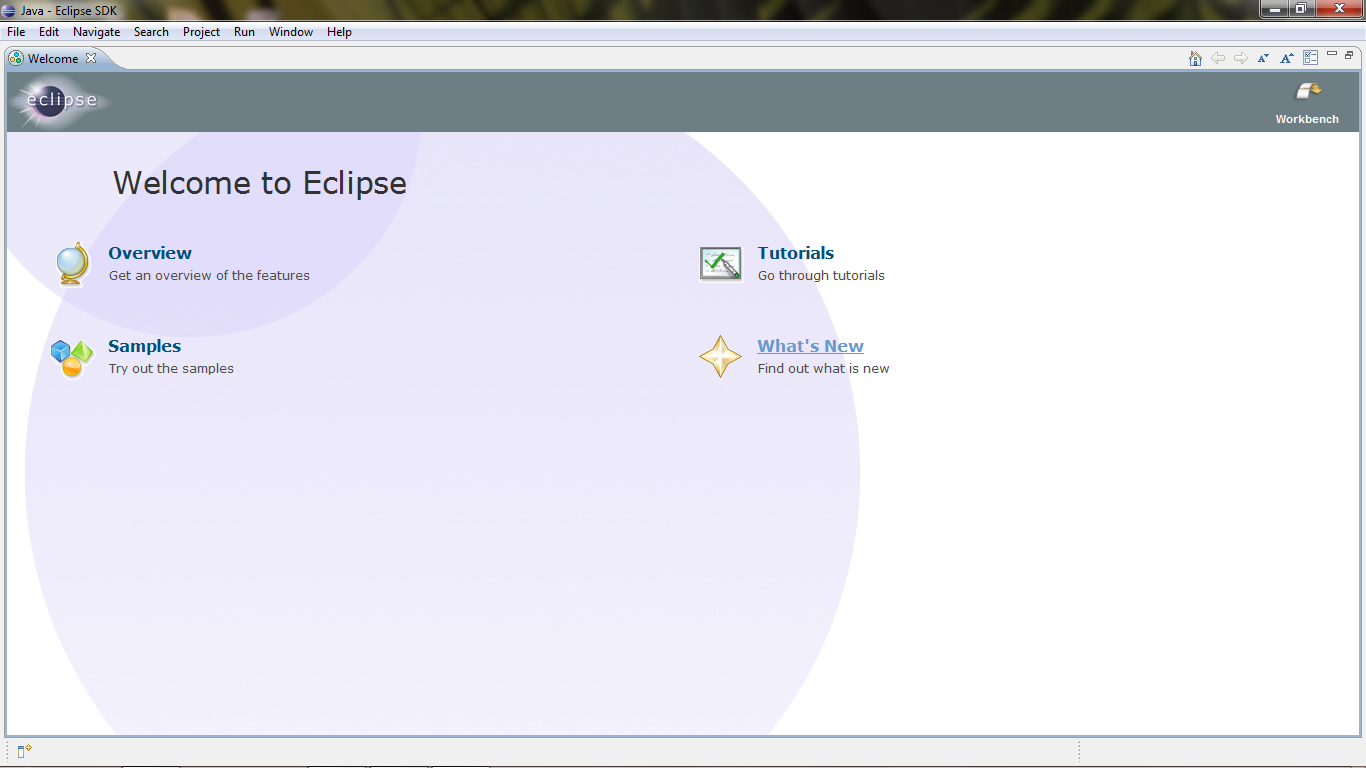
\includegraphics[width=0.7\textwidth]{images/eclipse_welcome.png}
\caption{Eclipse welcome screen}
\label{fig:welcome}
\end{figure}

\begin{figure}[H]
\centering
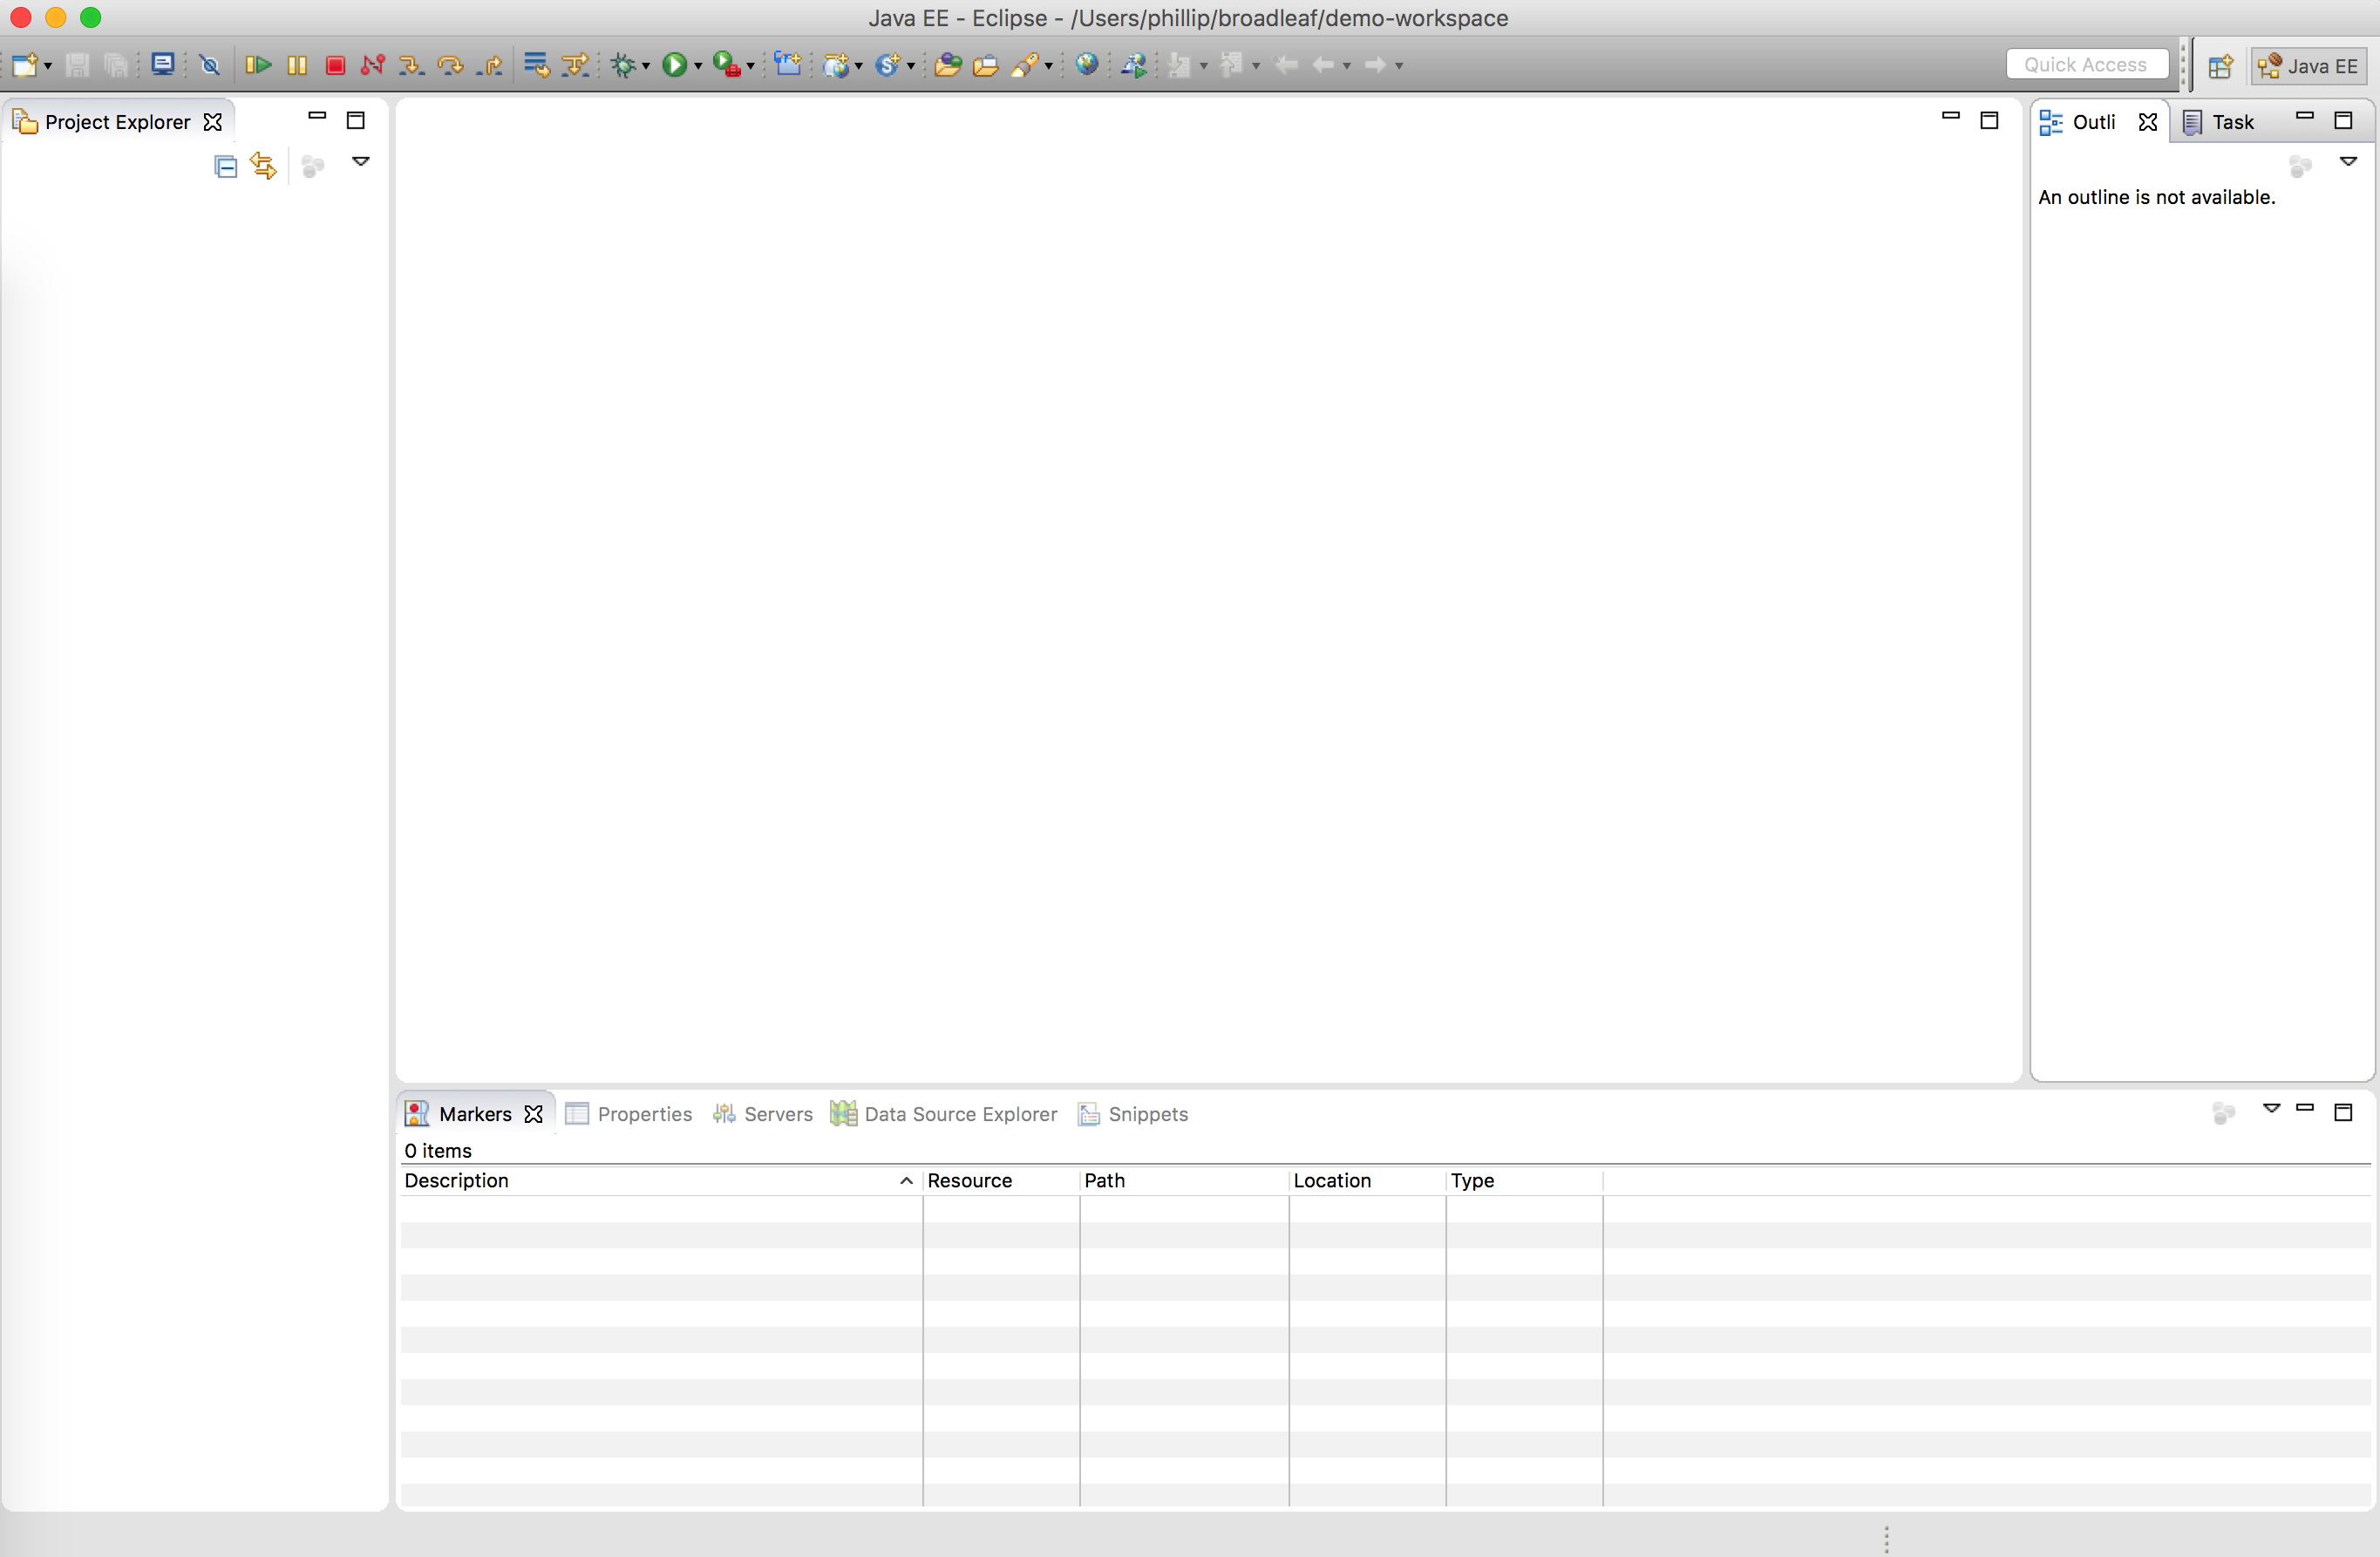
\includegraphics[width=0.7\textwidth]{images/eclipse_workspace.png}
\caption{Eclipse Workspace / Workbench}
\label{fig:workspace}
\end{figure}

To start a new project, click on \textbf{File --> New --> Java Project}. A dialog will appear. You should give your project a name, select a folder for it (optional), and click finish. You should see your project appear in the left hand dialog of the screen. If you expand the project, you should see a reference to your Java system library, as well as a folder called \textbf{src}. 

Your next task is create your first Java class. Right click on your project on the left and select \textbf{New --> Class}. A dialog will appear (see figure ~\ref{fig:newclass}), name your class \textbf{Power}, and select the check box that says \textbf{public static void main(String[] args)}. this option will create a main method automatically (though if you forget to do this, you can just type in the main method code manually).

\begin{figure}[H]
\centering
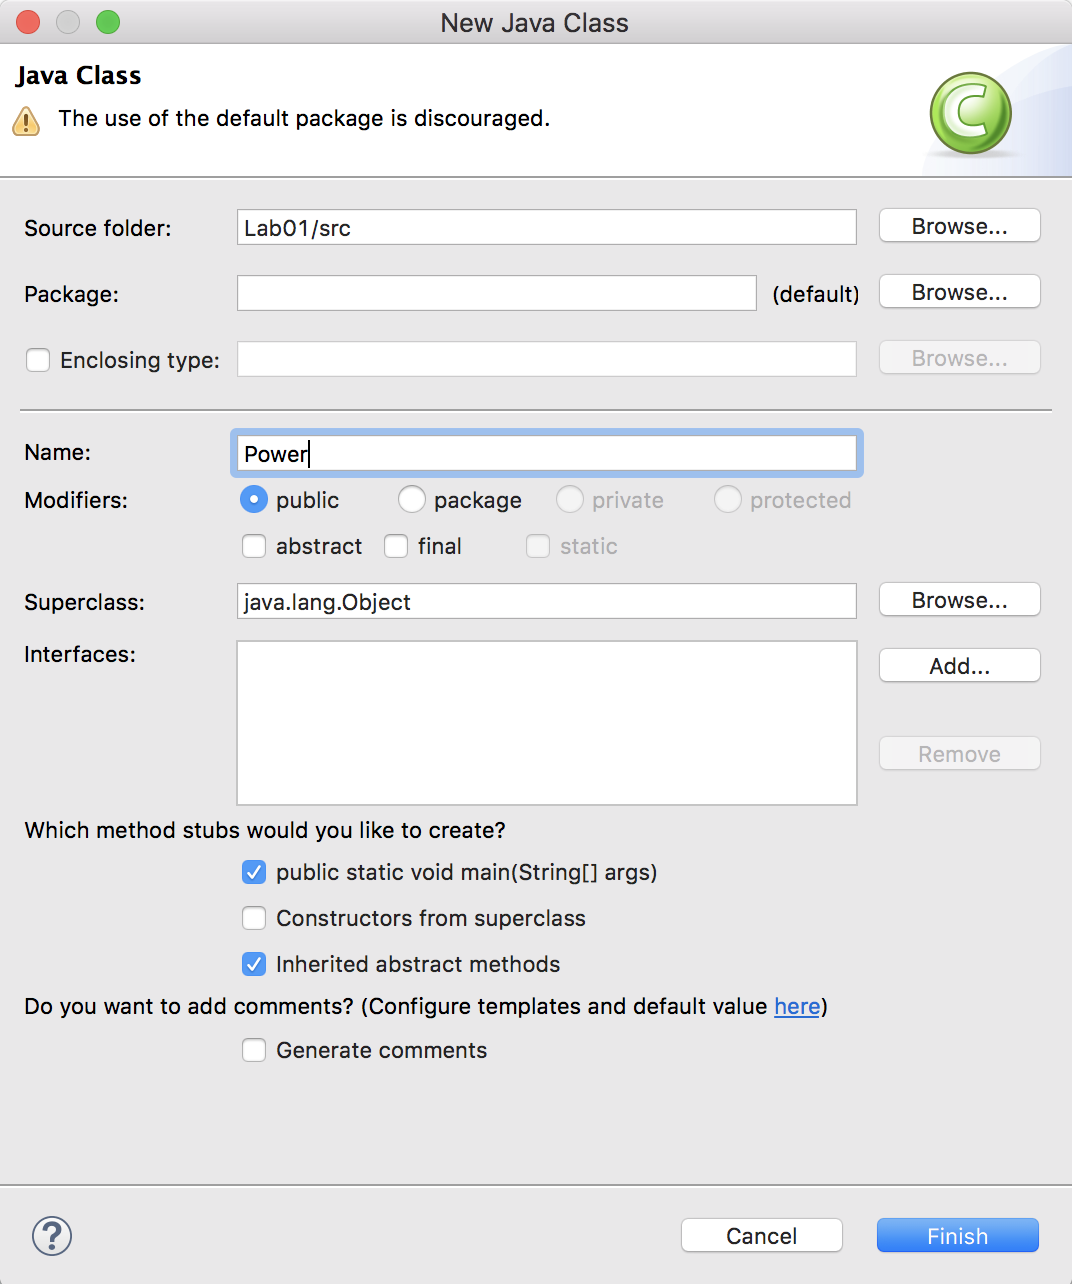
\includegraphics[width=0.4\textwidth]{images/eclipse_class_dialog.png}
\caption{New Class Dialog Screen}
\label{fig:newclass}
\end{figure}

You are ready to begin coding. For this homework, you will only need the one class, and you can write all of your code in this area. To run your program, there is a small green bug icon at the top of the screen. 


%------------------------------------------------

\subsection{Power.java}

Now that your environment is setup, you will write one very small Java method as a warm-up. The method signature is:

\begin{lstlisting}
public static long power(int base, int exp);
\end{lstlisting}

This method should accept two parameters (base and exp) and return the result of base to the power of exp. For example, \emph{power(2,3)} would return 8 because $2^3=8$. 

Your Power.java file should also contain a \emph{main method} to handle input and output. Your main method should take in two numbers from the user keyboard. First, the base and second, the exponent. Then, your program should invoke the power method above and present the user (via the console) the value of base to the exponent power. You can assume that when we test your code, all inputs will fit inside of int types, and all correct answers will fit inside of long types. This method may be iterative or recursive, but \textbf{may not use any library functions such as Math.pow()}.

\textbf{SAMPLE INPUT:}

\begin{lstlisting}
2
3
\end{lstlisting}

\textbf{SAMPLE OUTPUT:}

\begin{lstlisting}
8
\end{lstlisting}

\subsection{Gradescope}

You should submit your code to \emph{Gradescope}. If you are having trouble with your submission, you should double check the following common problems:

\begin{enumerate}
	\item Make sure you are only submitting one file, and it is called \emph{Power.java} (exactly, not power.java or pOwer.java).
	\item Make sure you remove any \emph{package} statements from your code before submitting. The autograder doesn't expect your file to be inside a package for this assignment.
	\item Make sure your output is in the correct format (see above) exactly. You should not be printing ANYTHING else or the autograder will think your output is incorrect.
\end{enumerate}



%------------------------------------------------

%----------------------------------------------------------------------------------------

\end{document}


%----------------------------------------------------------------------------------------
%----------------------------------------------------------------------------------------
%----------------------------------------------------------------------------------------
%----------------------------------------------------------------------------------------
%----------------------------------------------------------------------------------------
%----------------------------------------------------------------------------------------


%WORKS CITED:

%%%%%%%%%%%%%%%%%%%%%%%%%%%%%%%%%%%%%%%%%
% Short Sectioned Assignment
% LaTeX Template
% Version 1.0 (5/5/12)
%
% This template has been downloaded from:
% http://www.LaTeXTemplates.com
%
% Original author:
% Frits Wenneker (http://www.howtotex.com)
%
% License:
% CC BY-NC-SA 3.0 (http://creativecommons.org/licenses/by-nc-sa/3.0/)
%
%%%%%%%%%%%%%%%%%%%%%%%%%%%%%%%%%%%%%%%%%

%----------------------------------------------------------------------------------------
%	PACKAGES AND OTHER DOCUMENT CONFIGURATIONS
%----------------------------------------------------------------------------------------